Klasifikuojant daugiamačius duomenis susiduriame su taip vadinamu dimensiškumo
prakeiksmu (angl. curse of dimentionality). Pavyzdžiui, kai dimensijų skaičius įkopia į
trečią ar ketvirtą eilę naudoti paprastus klasifikavimo algoritmus tampa
nebeefektyvu nei laiko nei klasifikavimo našumo atžvilgiais. Vienas iš būdų
kovoti su dimensiškumo prakeiksmu
yra naudoti vienokius ar kitokius dimensijų skaičiaus mažinimo metodus. Šiame
skyriuje nagrinėsiu bazinius dimensijų atsirinkimo metodus, keletos 
kriterijų suliejimą metodą (angl.
feature selection based on multicriterion fusion)\cite{5611484}, bei
stabilių dimensijų grupių išskyrimo metodą\cite{Loscalzo:2009:CGS:1557019.1557084}.

\subsection{Baziniai dimensijų atrinkimo metodai}

Yra pasiūlyta daugybė dimensijų atrinkimo metodų. Šiame skyriuje aptarsiu
keletą taip vadinamų bazinių\footnote{Aptarsiu tik bazinius todėl, kad jie yra 
svarbiausi, nes jų tarpusavio rezultatai yra nekoreliuojantys, o nekoreliuojančius
rezultatus galima panaudot juos apjungiant, taip gauname sinergijos efektą.}
dimensijų atrinkimo metodų: 
\begin{enumerate}
 \item Fisher'io įvertis (angl. Fisher ratio)\cite{Pavlidis:2001:GFC:369133.369228};
 \item Atpalaidavimo metodas\cite{DBLP:journals/ml/Robnik-SikonjaK03} (ang. relief);
 \item Asimetrinis priklausomybės koeficientas\cite{Shannon:2001:MTC:584091.584093} (ADC) (angl.
 Asymmetric Dependency Coefficient);
 \item Absoliučių svorių SVM\cite{vapnik2000nature} (AW-SVM) (angl. Absolute Weight SVM)
 \item Rekursyvus dimensijų eliminavimas pagal SVM\cite{Guyon:2002:GSC:599613.599671} (SVM-RFE) (angl. Recursive
 Feature Elimination by SVM)
\end{enumerate}

\subsubsection{Fisher'io įvertis}

Fisher'io įvertis vertina indivualias dimensijas pagal jų klasių atskiriamąją 
galią. Dimensijos įvertis yra sudarytas iš tarpklasinio skirtumo santykio su 
vidiniu klasės pasiskirstymu:
\begin{equation}
 FR(j) = \frac{(\mu_{j1} - \mu_{j2})^2}{\sigma_{j1}^2 + \sigma_{j2}^2},
\end{equation}
kur, $j$ - yra dimensijos indeksas, $\mu_{jc}$ - dimensijos $j$ reikšmių vidurkis
klasėje $c$, $\sigma_{jc}^2$ - dimensijos $j$ reikšmių standartinis nuokrypis
klasėje $c$, kur $c={1,2}$. Kuo didesnis yra Fisher'io įvertis, tuo geriau ta
dimensija atskiria klases.

\subsubsection{Atpalaidavimo metodas}

Atpalaidavimo metodas iteratyviai skaičiuoja dimensijų ,,susietumą``. Pradžioje
,,susietumas`` visoms dimensijoms yra lygus nuliui. Kiekvienoje
iteracijoje atsitiktinai\footnote{Pastebėtina, kad metodas 
turi atsitiktinį elementą, todėl klasifikavimo ir  dimensijų atrinkimo stabilumo
rezultatai dažniausiai šiek tiek varijuoja.} pasirenkamas objektas iš duomenų
bazės, surandamas
artimiausi kaimynai iš tos pačios ir kitos klasės, ir atnaujinamos visų 
dimensijų ,,susietumo`` reikšmės. Dimensijos įvertis yra vidurkis visų objektų
atstumų iki artimiausių kaimynų iš tos pačios ir kitos kasės:
\begin{equation}
 W(j)=W(j) - \frac{diff(j, x, x_H)}{n} + \frac{diff(i, x, x_M)}{n},
\end{equation}
kur $W(j)$ - $j$-osios dimensijos ,,susietumo`` įvertis, $n$ - objektų aibės 
dydis,$x$ - atsitiktinai pasirinktas objektas, $x_H$ - artimiausias
kaimynas iš tos pačios klasės (angl. nearest-Hit), $x_M$ - artimiausias kaimynas
iš kitos klasės, $diff(j, x, x')$ - $j$-osios dimensijos reikšmių skirtumas
tarp laisvai pasirinkto objekto $x$ ir atitinkamo kaimyno, kur skirtumą į
intervalą $[0, 1]$ normalizuojanti funkcija yra:
\begin{equation}
 diff(j, x, x')=\frac{|x_j- x_j'|}{x_{j max} - x_{i min}},
\end{equation}
kur $x_{j max}$ ir $x_{j min}$ yra maximali ir minimali $j$-osios dimensijos
reikšmės. ,,Susietumo`` reikšmių atnaujinimas yra vykdomas $n$ kartų ir kuo
didesnė galutinė reikšmė, tuo svarbesnė dimensija.

\subsubsection{Asimetrinis priklausomybės koeficientas}

Asimetrinis priklausomybės koeficientas yra dimensijų reitingavimo motodika,
kuri matuoja klasės $Y$ etiketės (angl. label) priklausomybę pagal $j$-ąją
dimensiją, naudodama informacijos prieaugį (angl. information gain):
\begin{equation}
 ADC(Y, j) = \frac{MI(Y, X_j)}{H(Y)},
\end{equation}
kur $H(Y)$ - klasės $Y$ entropija, o $MI(Y, X_j)$ - yra bendrumo informacija
(angl. mutual information) tarp klasės etiketės $Y$ id $j$-osios dimensijos
\begin{equation}
 H(Y)=-\sum_y{p(Y=y)log{p(Y=y)}}, 
\end{equation}
\begin{equation}
 H(X_j)=-\sum_x{p(X_j=x) log{p(X_j=x)}},
\end{equation}
\begin{equation}
 MI(Y, X_j) = H(Y) + H(X_j) - H(Y, X_j),
\end{equation}
\begin{equation}
 H(Y, X_j) = -\sum_{y,x_j}{p(y, x_j)log{p(y, x_j)}},
\end{equation}

Kuo didesni ADC įverčiai, tuo dimensija yra svarbesnė, nes turi daugiau
informacijos apie duomenų klases.

\subsubsection{Absoliučių svorių SVM}

Atraminių vektorių metodas (SVM) ir vienas populiariausių klasifikavimo algortimų,
nes jis gerai susidoroja su daugiamačiais duomenimis. Yra keletas bazinių 
SVM variantų, bet šiame darbe naudosime tiesinį SVM, nes jis demonstruoja
gerus rezultatus dirbant su genų ekspresijos duomenimis. Tiesinis SVM yra
hiperplokštuma apibrėžta kaip:
\begin{equation}
 \sum_{j=1}^{p}{w_jx_j + b_0 = 0},
\end{equation}
kur $p$ - dimensijų kiekis, $w_j$ - j-osios dimensijos svoris, $x_j$ - j-osios
dimensijos kintamasis, $b_0$ - konstanta. Dimensijos absoliutus\footnote{Svorį
reikia imti absoliutaus dydžio, nes neigiamas svoris implikuoja priklausomybę 
vienai klasei, o teigiamas kitai klasei.} svoris gali būti panaudotas
dimensijų reitingavimui. Pastebėtina, kad svorių nustatymas yra atliekamas tik 
vieną kartą\footnote{SVM-RFE - metodas svorius nustato daug kartų.}.

\subsubsection{Rekursyvus dimensijų eliminavimas pagal SVM}

Rekursyvus diemnsijų eliminavimas pagal SVM yra vienas populiariausių dimensijų
atrankos algoritmų. Todėl, jis yra naudojamas, kaip atskaitos taškas vertinant
kitus dimensijų atrankos metodus. Iš esmės šis metodas yra daugkartinis 
absoliučių svorių SVM metodo taikymas nuolat išmetinėjant dimensijas su 
mažiausiais svoriais. Rekursyvus dimensijų eliminavimas mums padeda surasti 
tinkamą dimensijų poaibį, kas nevisada pavyksta su dimensijų reitingavimo 
metodais. Bendroji rekursyvaus dimensijų eliminavimo procedūra:
\begin{enumerate}
 \item Turime pilną dimensijų rinkinį $F_0$, nustatome $i=0$.
 \item Įvertiname kiekvienos dimensijos kokybę dimensijų aibėje $F_i$.
 \item Išmetame mažiausiai svarbią dimensiją iš $F_I$ tam, kad gautume
 dimensijų rinkinį $F_{i+1}$.
 \item Nustatome $i=i+1$ ir grįžtame į antrąjį žingsnį kol nėra patenkinta 
 algoritmo pabaigos sąlyga.
\end{enumerate}
Jei trečiajame algoritmo žingsnyje yra pašalinama tik viena dimensija, tai gauname dar
ir dimensijų reitingavimą, o jei pašalinamos kelios dimensijos ar jų dalis
(pvz. 50\%) tai reitingavimo negauname. Pastebėtina, kad rekursyvus dimensijų
eliminavimas gali labai padidinti algoritmo sudėtingumą skaičiavimo resursų
atžvilgiu. Algoritmo pabaigos sąlyga gali būti koks nors konkretus dimensijų
skaičius arba tiesiog dimensijų aibę mažinti tol, kol dimensijų visai nebeliks.


\subsection{Savybių pasirinkimo pagal keletos kriterijų suliejimą metodas}

Šio metodo esmė yra panaudoti kelis savybių atrinkimo metodus suliejant jų
rezultatus į vieną bendrą rezultatą. Kodėl naudinga sulieti keletą savybių
atrinkimo metodų? Sulieti keletą savybių atrinkimo metodų naudinga, nes
pavieniai savybių atrinkimo metodai be to, kad turi savitų privalumų, visada
turi ir savo silnybių, pavyzdžiui, jautrumas išimtims (angl. outliers), negali
rasti savybių tarpusavio priklausomybių, etc. Suliejant keletą skirtingų metodų
suliejamos gerosios pavienių savybių atrinkimo metodų savybės, taip
kompensuojant algoritmų silpnybes.

Galima pavienių savybių atrankos rezultatus sulieti pagal šias suliejimo
strategijas:
\begin{enumerate}
  \item Suliejimas pagal svorius
  \item Suliejimas pagal reitingus (angl. rank)
  \item Sulieti ir pagal svorius ir pagal reitingus
\end{enumerate}

Suliejimo pagal svorius būdu būtinai reikia atlikti svorių normalizavimą. Kitu
atveju savybių įvertinimo metodai bus nepalyginami. Pirmajame paveikslėlyje
nenormalizuotų svorių skiriasi netgi intervalai. Antrajame paveikslėlyje matoma,
kad net ir normalizavus svorius gana stipriai skiriasi svorių kvartiliai.

\begin{figure}[htb]
\begin{center}
\leavevmode
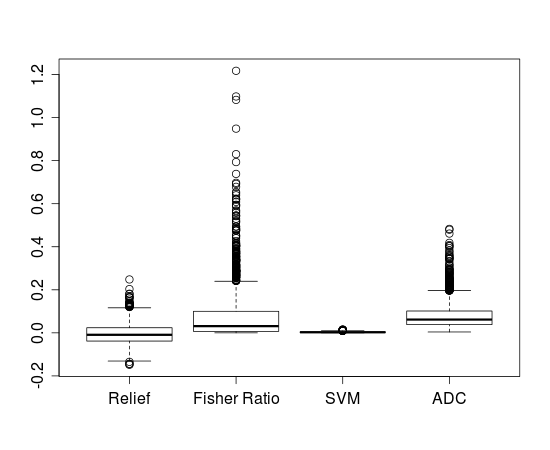
\includegraphics[width=0.5\textwidth]{images/boxplot_colon_all.png}
\end{center}
\caption{Pavienių savybių atrinkimo metodų nenormalizuotas svorių
pasiskirstymas.}
\label{fig:flash}
\end{figure}

\begin{figure}[htb]
\begin{center}
\leavevmode
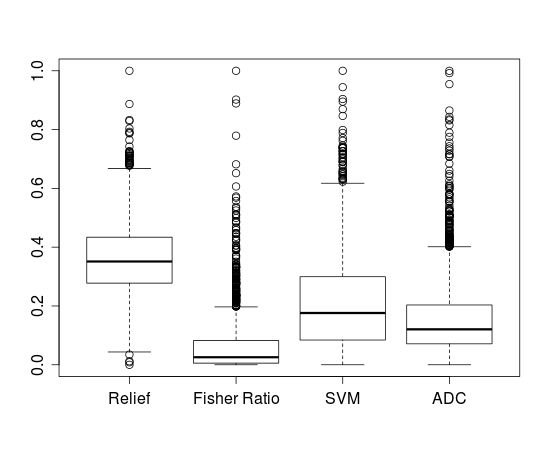
\includegraphics[width=0.5\textwidth]{images/boxplot_colon_all_normalized.png}
\end{center}
\caption{Pavienių savybių atrinkimo metodų normalizuotas svorių
pasiskirstymas.}
\label{fig:flash}
\end{figure}

Suliejimo pagal reitingus metodas nereikalauja normalizavimo, nes tiesiog imame
savybių svorių įverčius ir juos išrykiuojame mažėjimo tvarka - išreitinguojame.

Savybių įverčių pagal svorius ir reitingus metodas vyksta dviem žingsniais:
\begin{enumerate}
  \item suliejame savybes pagal svorius ir taip gauname vieną savybių reitingą,
  kurį prijungiame prie kitų savybių reitingų;
  \item reitinguojame savybes pagal visus turimus pavienius reitingus.
\end{enumerate} 
